\subsection{Web Application Security and Security Risks}
According to synopsys, the concept of \quotes{Web Application Security}
\begin{quote}
	involves a collection of security controls engineered into a Web application to protect its assets from potentially malicious agents. Web applications, like all software, inevitably contain defects. Some of these defects constitute actual vulnerabilities that can be exploited, introducing risks to organizations. Web application security defends against such defects. It involves leveraging secure development practices and implementing security measures throughout the software development life cycle (SDLC), ensuring that design-level flaws and implementation-level bugs are addressed.
\end{quote}
Developers and publishers of web applications are leveraging secure development practices to prevent security risks like those specified in the OWASP Top 10 document.
The OWASP Top 10 standard awareness document for developers and web application security represents a broad consensus about the most critical security risks to web applications.
It includes security risks based on vulnerabilities that could be exploited using malicious \acrshort{http} requests.
\cite{OWASP/Top10}

Broken Access Control is the top 1 security risk in the OWASP Top 10 list from 2021.
Broken Access Control enables users to act outside of their intended permissions.
Examples include access to undisclosed information, modification or destruction of data and performing business functions outside the users limits.
OWASP mentiones an attack scenario on an web application with broken access control where the attacker force browses to target URLs. \cite{OWASP/BrokenAccessControl,OWASP/Risks2021}

Force browsing is described by the OWASP Foundation as follows:
\begin{quote}
	Forced browsing is an attack where the aim is to enumerate and access resources that are not referenced by the application, but are still accessible.

	An attacker can use Brute Force techniques to search for unlinked contents in the domain directory, such as temporary directories and files, and old backup and configuration files. These resources may store sensitive information about web applications and operational systems, such as source code, credentials, internal network addressing, and so on, thus being considered a valuable resource for intruders.

	This attack is performed manually when the application index directories and pages are based on number generation or predictable values, or using automated tools for common files and directory names.

	This attack is also known as Predictable Resource Location, File Enumeration, Directory Enumeration, and Resource Enumeration.
	If the target URL corresponds to an admin page, admin privileges should be required to access the page. \cite{OWASP/forcebrowsing}
\end{quote}
If a user without admin privileges can access a page reserved for admins, the access control is broken. An example for Broken Access Control is given involving PhpMyAdmin.

PhpMyAdmin is a web application that allows users to manage MySQL databases over the web.
In some cases, the user interface of PhpMyAdmin can be accessed via the URL \verb|http://servername/phpmyadmin| after publishing the application via a web server. Single signon authentication is supported by PhpWebAdmin.
\cite{phpmyadmin/overview,phpmyadmin/quickinstall,ubuntu/phpmyadmin,phpmyadmin/signon}

The interface of PhpWebAdmin is intended to be accessed by an administrative audience.
If a user force browses to the specified URL and this page can be accessed by users without administrative privileges through misconfigured single sign on, it is a case of Broken Access Control.
As an additional security control in this case, a web application firewall could be used to prohibit any access to the URLs containing the path \verb|/phpmyadmin|.
If database administration is usually done locally, this would suffice.
Alternatively, a whitelist of remote addresses allowed to access \verb|/phpmyadmin| could be used in the web application firewall configuration.

%{\color{red} maybe add ssrf here: \\ \verb|https://owasp.org/Top10/A10_2021-Server-Side_Request_Forgery_\%28SSRF\%29/|}

Injection is the top 1 security risk in the OWASP Top 10 list from 2017.
An application is vulnerable to attack when, among others, user-input is incorrectly validated, sanitized or filtered by the application.
The OWASP Foundation mentiones the common weakness CWE-79: \acrfull{xss} as one of the weaknesses caused by incorrectly neutralized user-controllable input. \cite{OWASP/Risks2017,OWASP/Injection}

\begin{figure}
	\centering
	\includegraphics[width=0.85\textwidth]{reflxss.png}
	\caption{Visualization of Reflected XSS \cite{portswigger/reflxss}}
	\label{fig:reflxss}
\end{figure}

\acrlong{xss} vulnerabilities are described in the \acrfull{cwe} as follows:
\begin{quote}
	Cross-site scripting (XSS) vulnerabilities occur when:

	Untrusted data enters a web application, typically from a web request.
	The web application dynamically generates a web page that contains this untrusted data.
	During page generation, the application does not prevent the data from containing content that is executable by a web browser, such as JavaScript, HTML tags, HTML attributes, mouse events, Flash, ActiveX, etc.
	A victim visits the generated web page through a web browser, which contains malicious script that was injected using the untrusted data.
	Since the script comes from a web page that was sent by the web server, the victim's web browser executes the malicious script in the context of the web server's domain.
	This effectively violates the intention of the web browser's same-origin policy, which states that scripts in one domain should not be able to access resources or run code in a different domain.

	There are three main kinds of XSS:

	\textbf{Type 1: Reflected XSS (or Non-Persistent)} - The server reads data directly from the HTTP request and reflects it back in the HTTP response. Reflected XSS exploits occur when an attacker causes a victim to supply dangerous content to a vulnerable web application, which is then reflected back to the victim and executed by the web browser. The most common mechanism for delivering malicious content is to include it as a parameter in a URL that is posted publicly or e-mailed directly to the victim. URLs constructed in this manner constitute the core of many phishing schemes, whereby an attacker convinces a victim to visit a URL that refers to a vulnerable site. After the site reflects the attacker's content back to the victim, the content is executed by the victim's browser.

	\textbf{Type 2: Stored XSS (or Persistent)} - The application stores dangerous data in a database, message forum, visitor log, or other trusted data store. At a later time, the dangerous data is subsequently read back into the application and included in dynamic content. From an attacker's perspective, the optimal place to inject malicious content is in an area that is displayed to either many users or particularly interesting users. Interesting users typically have elevated privileges in the application or interact with sensitive data that is valuable to the attacker. If one of these users executes malicious content, the attacker may be able to perform privileged operations on behalf of the user or gain access to sensitive data belonging to the user. For example, the attacker might inject XSS into a log message, which might not be handled properly when an administrator views the logs.

	\textbf{Type 0: DOM-Based XSS} - In DOM-based XSS, the client performs the injection of XSS into the page; in the other types, the server performs the injection. DOM-based XSS generally involves server-controlled, trusted script that is sent to the client, such as Javascript that performs sanity checks on a form before the user submits it. If the server-supplied script processes user-supplied data and then injects it back into the web page (such as with dynamic HTML), then DOM-based XSS is possible.

	Once the malicious script is injected, the attacker can perform a variety of malicious activities. The attacker could transfer private information, such as cookies that may include session information, from the victim's machine to the attacker. The attacker could send malicious requests to a web site on behalf of the victim, which could be especially dangerous to the site if the victim has administrator privileges to manage that site. Phishing attacks could be used to emulate trusted web sites and trick the victim into entering a password, allowing the attacker to compromise the victim's account on that web site. Finally, the script could exploit a vulnerability in the web browser itself possibly taking over the victim's machine, sometimes referred to as "drive-by hacking."

	In many cases, the attack can be launched without the victim even being aware of it. Even with careful users, attackers frequently use a variety of methods to encode the malicious portion of the attack, such as URL encoding or Unicode, so the request looks less suspicious. \cite{mitre/XSS}
\end{quote}

\begin{figure}
	\centering
	\includegraphics[width=0.9\textwidth]{storedxss.png}
	\caption{Visualization of Stored XSS \cite{acunetix/storedxss}}
	\label{fig:storedxss}
\end{figure}

Reflected \acrshort{xss} is visualized in Figure~\ref{fig:reflxss}, Stored \acrshort{xss} is visualized in Figure~\ref{fig:storedxss}, DOM-Based \acrshort{xss} is visualized in Figure~\ref{fig:domxss}.

As an additional protection mechanism, web application firewalls can be used to block \acrshort{xss} payloads in \acrshort{http} requests. In web applications, where script code transmission is not part of the business, the rules intended to block requests containing \acrshort{xss} payloads could be pretty strict.

\acrshort{xss} payloads will be the main payloads tested in the proceeding of this work.
\acrshort{xss} weaknesses represent only a fraction of possible weaknesses in web applications. Therefore, to achieve a comprehensive understanding of a web applications attack surface, research into further kinds of typical web application weaknesses should be considered.

When employing a web application firewall as an additional protection mechanism, the Defense-in-Depth strategy is followed.
The first layer of defense should be the counter measures built into the web application, like proper access control and neutralization of user-input.
An additional layer of defense is then put on top by employing a web application firewall.
If a misconfigured security control in the web application failes to correctly handle a specific malicious request, there is a chance that the web application firewall is configured in a way that detects and blocks the malicious request before it can reach the web application and cause an incident.
Avoiding security incidents with the Defense-in-Depth strategy corresponds to
\begin{quote}
	the application of multiple countermeasures in a layered or stepwise manner to achieve security objectives. The methodology involves layering heterogeneous security technologies in the common attack vectors to ensure that attacks missed by one technology are caught by another.
\end{quote}
as defined by the \acrfull{nist}. \cite{nist/did}

% \begin{figure}
% 	\centering
% 		\includegraphics[width=0.95\textwidth]{domxss.jpg}
% 	\caption{Visualization of DOM-Based XSS \cite{cyberpunk/domxss}}
% 	\label{fig:domxss}
% \end{figure}



\begin{figure}
	\centering
	\tikzmath{
		\au = 6.5; \vo = 3.5;
	}
	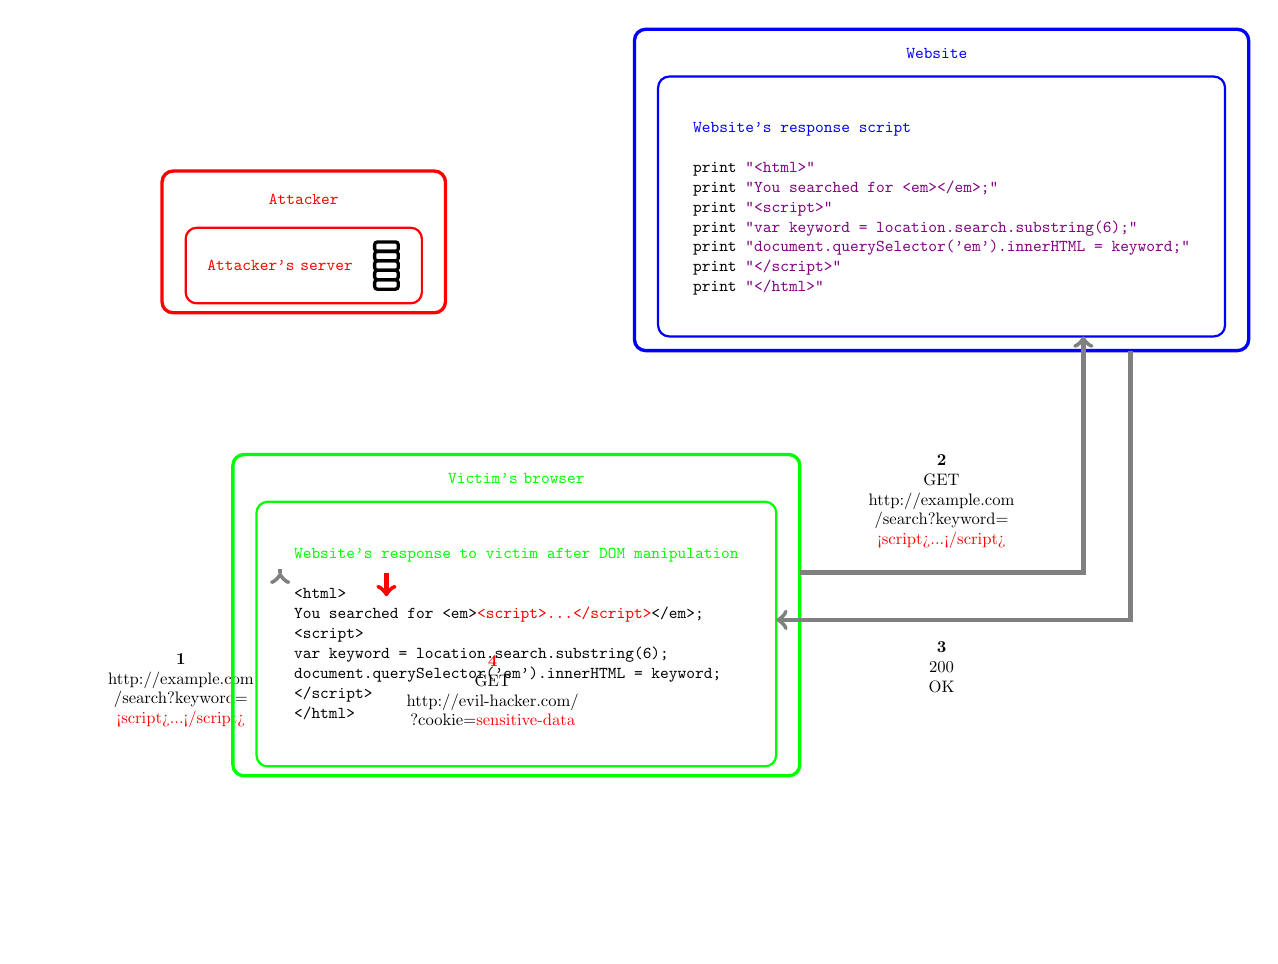
\begin{tikzpicture}[thick,scale=0.6, every node/.style={scale=0.6}]
		\begin{scope}[shift={+(0,1.5)}]
			\draw[red, very thick, rounded corners] (-3.5,5) rectangle (2.5,8.0);
			\draw[red, thick, rounded corners] (-3,5.2) rectangle (2,6.8);
			\node (a1)[red, align=left, font=\ttfamily, text width=5cm, text centered] at (-0.5,7.4) {\textbf{Attacker}};
			% \draw[black, very thick, rounded corners] (-1.5,7) rectangle (0.5,8);
			\node (a2)[red, align=left, font=\ttfamily, text width=4cm, text centered] at (-1,6) {\textbf{Attacker's server}};
			\foreach \y in {0,0.2,0.4,0.6,0.8}{
					\draw[black, very thick, rounded corners=1pt] (1.5,5.5 + \y) rectangle (1,5.7 + \y);
				}
		\end{scope}

		% attacker - victim
		\begin{scope}
			\draw[->, red, ultra thick] (1.25,\vo) -- (1.25,\au + 0.5);
			\draw[<-, gray, ultra thick] (-1,\vo) -- (-1,\au);
			\node[black, align=left, text width=10cm, text centered, circle] at (3.5,\au - 1.5)
			{
			{\color{red}
					\textbf{4}}\\
			GET\\
			http://evil-hacker.com/\\ 
			?cookie={\color{red}sensitive-data}
			};
			\node[black, align=left, text width=6cm, text centered, circle] at (-3.1,\au - 1.5)
			{
			\textbf{1}\\
			http://example.com\\
			/search?keyword=\\
			{\color{red}<script>...</script>}
			};
		\end{scope}

		% Victim
		\begin{scope}[shift={+(0,0)}]
			\draw[green, very thick, rounded corners] (-2,-3.3) rectangle (10,3.5);
			\draw[green, thick, rounded corners] (-1.5,-3.1) rectangle (9.5,2.5);
			% \draw[black, thick, rounded corners] (3,2.7) rectangle (5,3.7);
			% \draw[black, thick, rounded corners] (3,3.5) -- (5,3.5);
			\node[green, align=left, font=\ttfamily, text width=5cm, text centered] at (4,3) {\textbf{Victim's browser}};
			\node[black, align=left, font=\ttfamily] at (4,-0.3)
			{
				{\color{green}\textbf{Website's response to victim after DOM manipulation}}\\\\
				<html>\\
				You searched for <em>{\color{red}<script>...</script>}</em>;\\
				<script>\\
				var keyword = location.search.substring(6);\\
				document.querySelector('em').innerHTML = keyword;\\
				</script>\\
				</html>
			};
		\end{scope}

		% Website
		\begin{scope}[shift={+(9,8)}]
			\draw[blue, very thick, rounded corners] (-2.5,-2.3) rectangle (10.5,4.5);
			\draw[blue, thick, rounded corners] (-2,-2) rectangle (10,3.5);
			\node[blue, align=left, font=\ttfamily, text width=5cm, text centered] at (3.9,4) {\textbf{Website}};
			\node[black, align=left, font=\ttfamily] at (4,0.7)
			{
				{\color{blue}\textbf{Website's response script}}\\\\
				print {\color{violet}"<html>"}\\
				print {\color{violet}"You searched for <em></em>;"}\\
				print {\color{violet}"<script>"}\\
				print {\color{violet}"var keyword = location.search.substring(6);"}\\
				print {\color{violet}"document.querySelector('em').innerHTML = keyword;"}\\
				print {\color{violet}"</script>"}\\
				print {\color{violet}"</html>"}
			};
		\end{scope}

		% victim - website
		\begin{scope}
			\draw[->, gray, ultra thick] (10,1) -- (16,1) -- (16,6);
			\draw[<-, gray, ultra thick] (9.5,0) -- (17,0) -- (17,5.7);
			\node[black, align=left, text width=5cm, text centered] at (13, 2.5)
			{
			\textbf{2}\\
			GET \\
			http://example.com\\
			/search?keyword=\\
			{\color{red}<script>...</script>}
			};
			\node[black, align=left, text width=5cm, text centered] at (13, -1)
			{
				\textbf{3}\\
				200 \\
				OK
			};
		\end{scope}
	\end{tikzpicture}

	\caption{Visualization of DOM-Based XSS \cite{cyberpunk/domxss}}
	\label{fig:domxss}
\end{figure}
